\documentclass[twoside, final, 11pt]{articleMine}
\usepackage[english]{babel} \usepackage{a4wide}
\usepackage{amsmath,amssymb,accents} \usepackage{epsfig}
\usepackage{subfigure} \usepackage{units} \usepackage{graphicx}
\usepackage[displaymath, mathlines, right]{lineno} \usepackage{xspace}
\usepackage{color} \usepackage{epic,eepic,pstricks}
\usepackage{acronym} \usepackage{wrapfig,multicol}
\usepackage{deluxetable} \usepackage{todonotes} 
\usepackage{multirow}
\usepackage{url}
%\usepackage{slashbox}
\usepackage{lmodern} 
%\usepackage{caption}
\linenumbers
%\usepackage{showlabels}
\usepackage[draft]{showkeys}

%\usepackage[nolists, tablesfirst]{endfloat}
\graphicspath{{plots/}}
\newcommand*\patchAmsMathEnvironmentForLineno[1]{%
  \expandafter\let\csname old#1\expandafter\endcsname\csname #1\endcsname
  \expandafter\let\csname oldend#1\expandafter\endcsname\csname end#1\endcsname
  \renewenvironment{#1}%
     {\linenomath\csname old#1\endcsname}%
     {\csname oldend#1\endcsname\endlinenomath}}%
\newcommand*\patchBothAmsMathEnvironmentsForLineno[1]{%
  \patchAmsMathEnvironmentForLineno{#1}%
  \patchAmsMathEnvironmentForLineno{#1*}}%
\AtBeginDocument{%
\patchBothAmsMathEnvironmentsForLineno{equation}%
\patchBothAmsMathEnvironmentsForLineno{align}%
\patchBothAmsMathEnvironmentsForLineno{flalign}%
\patchBothAmsMathEnvironmentsForLineno{alignat}%
\patchBothAmsMathEnvironmentsForLineno{gather}%
\patchBothAmsMathEnvironmentsForLineno{multline}%
}
%\AtBeginFigures{\cleardoublepage}
%%%%%\parindent 5pt  
\parskip 1.2pt           % sets spacing between paragraphs
\def\Offline{\mbox{$\overline{\rm
Off}$\hspace{.05em}\raisebox{.4ex}{$\underline{\rm line}$}}\xspace}
\def\OfflineB{\mbox{$\bf\overline{\rm\bf
Off}$\hspace{.05em}\raisebox{.4ex}{$\bf\underline{\rm\bf line}$}}\xspace}

\def\eq#1{\begin{equation}#1\end{equation}}
%\def\al#1{\begin{align}#1\end{align}}
%\def\vc#1{{\bf #1}}
\def\pt#1{\accentset{\rightharpoonup}{#1}}
\include{myabbr}

\newcommand{\HRule}{\rule{\linewidth}{0.5mm}}
\newcommand{\VEM}{\mbox{VEM}}
\newcommand{\m}{\mbox{m}}

\let\stdsection\section  
%\renewcommand\section{\newpage\stdsection}  
 
\begin{document}

%\setpagewiselinenumbers
\modulolinenumbers[2]

%\linenumbers


\renewcommand\linenumberfont{\small\rmfamily}
\begin{center}
  \vspace*{-13ex}

  \rule{\linewidth}{0.1mm} \\[17mm] {\huge  EASIER}
     \begin{flushright}
       \small 
     
     \end{flushright}

  % 
\end{center}
% 
\vspace*{2ex} 
%
\thispagestyle{empty}
\noindent
\begin{abstract}
  \noindent

We present the instrumental development of EASIER, a radio detector of
cosmic ray, tuned  in the C-band (3.4-4.2 GHz) and  integrated into the
surface detector  of the Pierre  Auger Observatory. EASIER  intends to
observe the  Molecular Bremsstrahlung  Radiation (MBR) produced  by the
ionization electrons of the air shower  and in this way to measure its
longitudinal profile  with a full  duty cycle. Current  measurement of
the electromagnetic component lack of statistics at the highest energy
either due to reduced duty  cycle, fluorescence measurement, or due to
a  limited  spatial  extension  of  the signal,  beamed  component  of
radio. We developed  a radio detector in the  C-band working in slave
mode with the  Pierre Auger Observatory to probe  the intensity of the
MBR.  Two setups  were implemented following the evolution  of the MBR
theoretical expectations.  We present  the details of these setups and
their  calibrations   to  estimate  the  sensitivity   of  the  EASIER
experiment.

%% longitudinal profile  measurement make  use of the  fluorescence light
%% and are  thus limited  to at  most 15\% of  duty cycle  while previous
%% radio experiment measure a radio  signal beamed around the shower axis
%% thus not suited for a long distance
%%  component  , a  mass  sensitive measurement  through.
%% would  allow  for  the  measurement  of the  UHECR  mass  composition.
%% Previous observation of an isotropic radiation from an electromagnetic
%% shower in  laboratory experiment motivated  this study in  the C-band.
%% We show in this paper two versions of the detector

%%  The main purpose of
%% EASIER is the observation of the longitudinal profile of extensive air
%% shower at  microwave frequency.  Such observation would  allow for the
%% measurement of the  nature of the primary cosmic  ray, a key parameter
%% to pin point the physical  processes during their production and their
%% propagation  in  universe.      \\We first describe  the design
%% and  the instrumental characteristics  of EASIER.  We then  report the
%% first  observations made  out of  the EASIER  data. In  particular, we
%% report the  observation of  a clear signal  at microwave  frequency in
%% coincidence  with the  detection of  air  shower by  the Auger  array.
%% However the characteristics of  the observed signal, non isotropically
%% emitted and concentrated within 300m from the shower axis, don't match
%% the  expected  isotropic  emission.   Hence,  we  also  set  the  most
%% constraining limits on MBR from extensive air shower.
\end{abstract}

%
\thispagestyle{empty}
%$\;$
%\listoftodos
%\newpage
\noindent
\section*{Introduction}
The  origin of  Ultra  High  Energy Cosmic  Rays  (UHECRs) remains  an
unsolved question.  The  interpretation of the abrupt fall off  at the end of the           observed           spectrum          (E           $\geq$
\unit[5$\cdot10^{19}$])\cite{Fukushima:2013yea} is still being debated. It could result from the extinction of sources if the acceleration at source has reached its maximum energy, but can be interpreted as well as the result of the interaction of UHECR with background light, the GZK effect. The measurement of the composition of UHECR at the highest energies is of essential to disentangle between these two scenarios{ref}.\\ The UHECR are detected through the cascade of particles they induce in  the atmosphere, the Extensive Air Shower or EAS, over a large surface of collection to compensate for a very low flux of primary cosmic ray. For instance, the Pierre Auger Observatory is instrumented over \unit[3000]{km$^2$}. The two main techniques to detect EAS currently implemented are:
\begin{itemize}
\item  the  detection of  the EAS  front at   ground  by  an  array  of  particle  detectors (with  a  spacing  of   \unit[1.5]{km} for the Pierre Auger Observatory).
\item  the observation  of the  fluorescence light  emitted  along the
  shower development by the desexcitation of $N_2$ molecules.
\end{itemize}
One can infer the mass composition through various parameters of the extensive air shower. The position of its maximum of development, $\rm X_{max}$, is measured with the fluorescence technique and provides currently the best information on the mass composition but it is limited by the observation time the fluorescence detectors which can operate only during clear   moonless   night   i.e.    $\sim$   10$\%$ of the time. Other mass sensitive parameters are found with improved data analysis of the surface detector data, like the muon production depth~\cite{augermassmpd} or signal  asymmetry,  but these methods still show some limitations in terms of precision and model dependence. The upgrade undertaken by the Pierre Auger Collaboration aims at the measurement of the mass composition using the information of an additional scintillator allowing for the separation of muonic and electromagnetic components of the shower. An alternative solution would be the measurement of the EAS electromagnetic longitudinal profile with a 100\% duty cycle. This would allow for the estimation of two mass sensitive parameters: $\rm X_{max}$ and the ratio of the muonic and electromagnetic components by combination with the particle detector.
%
%The distribution of the shower energy among the electromagnetic and muonic components is another observable related to the mass composition.

% The combination of a particle measurement at ground with the measurement of the longitudinal profile through the radio component would provide two observables related to the mass composition measurement, enabling the measurement of the primary mass with an almost 100\% duty cycle.
In this perspective, the observation  of radio  waves  from  EAS  is an interesting technique. Firstly  proposed  and implemented in the 1960's  \cite{jelley65}, the radio detection,  of air shower is now  a well established technique mostly exploited in    the   VHF    band~\cite{huegeradioreview}.     In this band it was    shown in~\cite{augerradio} that the observed radiation is mainly produced by
the acceleration  of the  electrons of the  shower in  the geomagnetic
field, and in a smaller portion by the moving charge excess (also know
as Askaryan radiation).  However,  both of these radiations are beamed
forward in the  Cherenkov cone, which is around $\sim$ 1deg.  in  air, and centered around the shower axis.  The resulting  imprint of the radio signal at ground level is generally observable up to a few hundred meters limiting this
technique to densely instrumented  array therefore to primary energies of cosmic rays of around \unit[$10^{18}]{eV}$. The observation of the radio signal at larger distances would allow for sparser installation of detectors and make this technique also efficient at higher energies. This requires the ability to lower the detection threshold, a difficult task because of the radio frequency noise, including man made noise.  \\In 2008, a beam experiment detected
a signal  at microwave  frequencies (1.5-6 GHz) upon  the passage  of a
shower  of  charged particles  in  an anechoic  chamber~\cite{Gorham}.
This signal was interpreted  as Molecular Bremsstrahlung Radiation (MBR) and
its  intensity,  when extrapolated  to  air  shower  energy, could  be
detected in air shower with rather simple radio-detector systems.  The
MBR is produced by the acceleration of the ionization electrons in the
field  of the  molecules  in  the atmosphere.   The  intensity of  the
radiation is directly related with deposited energy by the shower
along the  atmosphere.  The measurement  of the time evolution  of the
radiation would allow one to determine the longitudinal development of
the shower, and the total received  power to measure the energy of the
primary particle.  Furthermore one expects  the intensity of MBR to be
emitted isotropically  and decrease with  the distance squared  and to
extend   further   than  the   previously   detected  radiation   like
geosynchrotron or Askaryan radiation. Finally, the equipment in this range of frequency has already been well developed for other application and can be found for a rather cheap price.\\ This results and the promising features  of  the MBR needed confirmation and led  to  the  development of  beam  experiments \cite{amy}, \cite{maybe}, as well as in situ experiments aiming at the direct  observation  from   air  showers  \cite{midas},  \cite{crome}, \cite{amber}.  In parallel, improved  calculations of the MBR produced by  air  shower  \cite{imen2016}  have  shown that  the  intensity  is exptected to  be lower by at  least two orders of  magnitude.\\ In this
paper, we  present the developments  of EASIER: Extensive Air Shower Identification with Electron Radiometer, a concept of radio detectors  integrated to the Pierre Auger Observatory  Surface Detector (SD). An EASIER detector is radio antenna combined with an envelope detector  installed on a SD station and is triggered with it. Thanks to the triggered mode, the Radio Frequency Interference (RFI)  and especially the man made noise is filtered out and allow for a reduced detection threshold. Thus this setup has the capability to probe the radio signal from UHECRs at large distances from the shower axis.  After the description of the general experimental setup, we details the calibration of two versions implemeted in the C-band ($\rm [3.4 - 4.2] GHz$), the first one EASIER61 is based on the original  estimation of the MBR and the second, GIGADuck, is an improved version with a better sensitivity. We then describe the  method to simulate  the MBR signal and apply it to the EASIER setups to estimate their expected performances.


% LocalWords:  UHECR

\section{EASIER}
EASIER is a radio detector concept, it is composed of a radio sensor and an adaptation electronics embedded in the surface detector of the Pierre Auger Observatory, its main component are sketched on the Fig.~\ref{fig:diagram}. This concept was implemented in three bandwidths: the VHF band (30-80 MHz), the L band (1-1.5GHz) and the C-band (3.4-4.2GHz). We focus in this article only on the C-band. The  EASIER experiment  is one  of the  three C-band experiments  deployed at  the  Pierre Auger  Observatory site  besides AMBER~\cite{Gorham} and MIDAS~\cite{midas}. All of these setups intend to observe the molecular Bremsstrahlung radiation emitted from the ionization electrons of the shower. Contrary to AMBER and MIDAS which instrument an array of feed  horn antennas illuminated by a parabolic  dish, EASIER  relies on the observation of the shower  from the  ground with  a wide  angle antenna  pointing up in the sky.
A first array of 61 antennas called EASIER61 is running  since  2011 and has reported the observation of radio signals from EAS but at small distances from the shower axis. New estimations of the expected intensity led us to implement a new array, called GIGADuck, with an enhanced sensitivity installed since March 2015. These arrays are presented in this section.  
\subsection {The noise environment in the Pierre Auger Observatory site}
Radio measurement are often hindered by man made noise. Prior to  the installation,  we made sure that the environment at the Pierre Auger Observatory was radio quiet in the C-band.  The Fig.~\ref{fig:Pampa_spec} shows the noise spectrum measured  with  a C-band  LNBf  in the  Pampa Amarilla. The gain of the amplifier used is roughly \unit[60]{dB}, the background noise is thus around \unit[-180]{dBm/Hz} in the band. No strong peak is observed above this level in the tens of spectra recorded.
 \begin{figure}[!h]
  \center {
  \subfigure{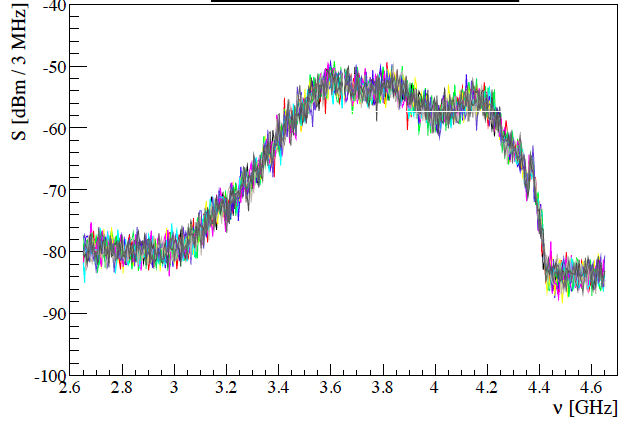
\includegraphics[width=0.49\linewidth]{Pampa_spec}}
    \subfigure{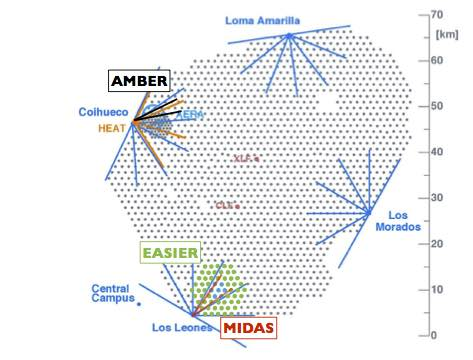
\includegraphics[width=0.49\linewidth]{augerarray.jpg}}  
  \caption{\small{Left:Frequency spectra in the C-band recorded in Pampa Amarilla. (The amplifier gain is around 60dB). Right: Footprint of EASIER array phase 1 (blue dots) and phase 2 (green dots).}}
  \label{fig:Pampa_spec}
    } 
\end{figure}

\subsection{The experimental setup}  
The basis of the EASIER detector is the  Pierre Auger  Observatory surface  detector. The Pierre Auger SD is  composed  of 1660 local stations arranged  in a tringular grid of  1500m spacement (see Fig.~\ref{fig:Pampa_spec}). Each local station is a water  Cherenkov detector equipped with three PMTs, a       local        acquisition       and       a       communication system, see~\cite{augerdetector} for a comprehensive description. An EASIER detector unit is designed to be integrated  into the  SD station.
 The receiver is a commercial horn antenna (Fig.~\ref{fig:detector}) made
 of a  feed and a  quarter wave length  monopole at its bottom.   It is
 tuned  for  a  central  frequency  of  3.8  GHz  and  a  bandwidth  of
 approximately \unit[500 to 800]{MHz}.  It  is associated with a low  noise block (LNB)  which amplifies  the signal by approximately  \unit[60]{dB} and lowers
 down the  central frequency to  \unit[1.35]{GHz}. The antenna and the LNB will be refered to LNBf within this document. A bias  tee is  inserted to provide  the power  supply to the  LNB and operate   the   transmission   of   the   RF  signal   on   a   single \unit[75]{$\Omega$} line.  Depending on  the setup, the line impedance  is adapted to \unit[50]{$\Omega$} by a resistor bridge.
 %% inducing a loss of  \unit[5.7]{dB}. 
 Potential low  frequency noises are filtered out  by a \unit[900]{MHz}
 high pass filter.  A logarithmic amplifier (minicircuit AD8318) serves
 as  a power  detector and outputs  a voltage  proportional to  the
 logarithm of the RF input power.   This model was chosen for its large
 frequency  bandwidth and  a fast  time response  of $\simeq$\unit[tens
   of]{ns} nominally.  This voltage is  in turn adapted to fit into  the local station  front  end, originally built to accept  PMT's negative voltage between 0 and
  -2V.  The EASIER  final analogic signal replaces one  of the low gain
  channel of  the local station (each local  station acquires ordinarly
  the last  dynode and the  anode of three  PMTs, the anode  being used
  only  in  case of  saturation  of the  dynode).   The  final part  of
  acquisition includes an antialiasing filter cutting frequencies above
  \unit[20]{MHz} and the FADC digitizer sampling a \unit[19.2]{$\mu$ s}
  waveform at a  \unit[40]{MHz} rate and coding the  analogic signal on
  10 bits~\cite{augertechnical}.   The data stream is then  sent to the
  central acquisition and the  reconstruction of the event is performed
  independently of the radio signal. As a consequence, no separated trigger for the radio signal is needed and the EASIER data are simply part of the regular SD data stream.  As  an additional benefit, the radio detector
is  powered by the  station battery  and is  also integrated  into the SD station's monitoring  system. 

\begin{figure}[!ht]
  \centering
  \hspace*{-3ex}  
  \subfigure{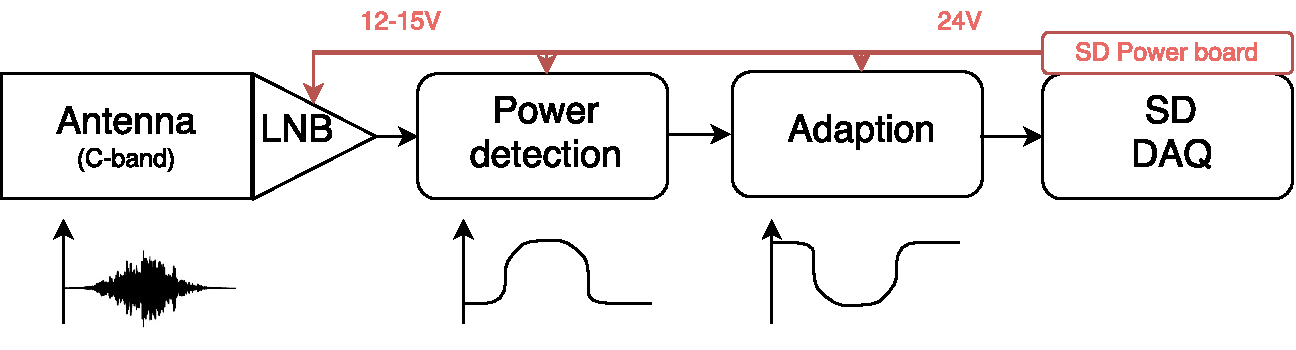
\includegraphics[width=0.69\linewidth]{blockdiagram.pdf}}  
  \caption{block diagram of an EASIER detector unit}
  \label{fig:diagram}  
\end{figure}

\subsubsection*{EASIER61}
A first  array of  seven detectors was  installed at the  Pierre Auger
Observatory  in April  2011.  The  good operation  and results  of this
first test  bed led to an  extension of 54 more  detectors covering a total
instrumented surface  of \unit[91]{$\rm km^2$}.  The  type of antenna used for
this setup  is a  commercial cylindrical horn  antenna with  a maximum
gain of around 9dB, it points to  the zenith and has a half power beam
width (HPBW)  of 90 degrees. The  first seven LNBf are  of the model GI301
made by Global Intersat and  the 54 units of the extension are from
WSInternational, model DMX241. The sensors, composed of the antenna and
the amplification system,  are installed on top of  the SD station (cf
Fig.~\ref{fig:detector} left) and the electronics box is located below
the hatch  box on top  of the SD  electronics.  The EASIER61  array is
located in  the south west part  of the Pierre  Auger Observatory, its
footprint is  shown in Fig.~\ref{fig:detector} (right).   On the total
of  61   antennas,  33  have   a  North-South  polarization,   and  28
East-West.\\ Several radio events in coincidence with an  EAS were measured  with EASIER61 which validated the concept. However, the distance from the antenna to the shower axis of these events are of the order of a few hundreds of meters, thus they can be also attributed to a coherent emission like the ones measured at lower frequency.
\begin{figure}[!ht]
  \centering
  \hspace*{-3ex}  
  \subfigure{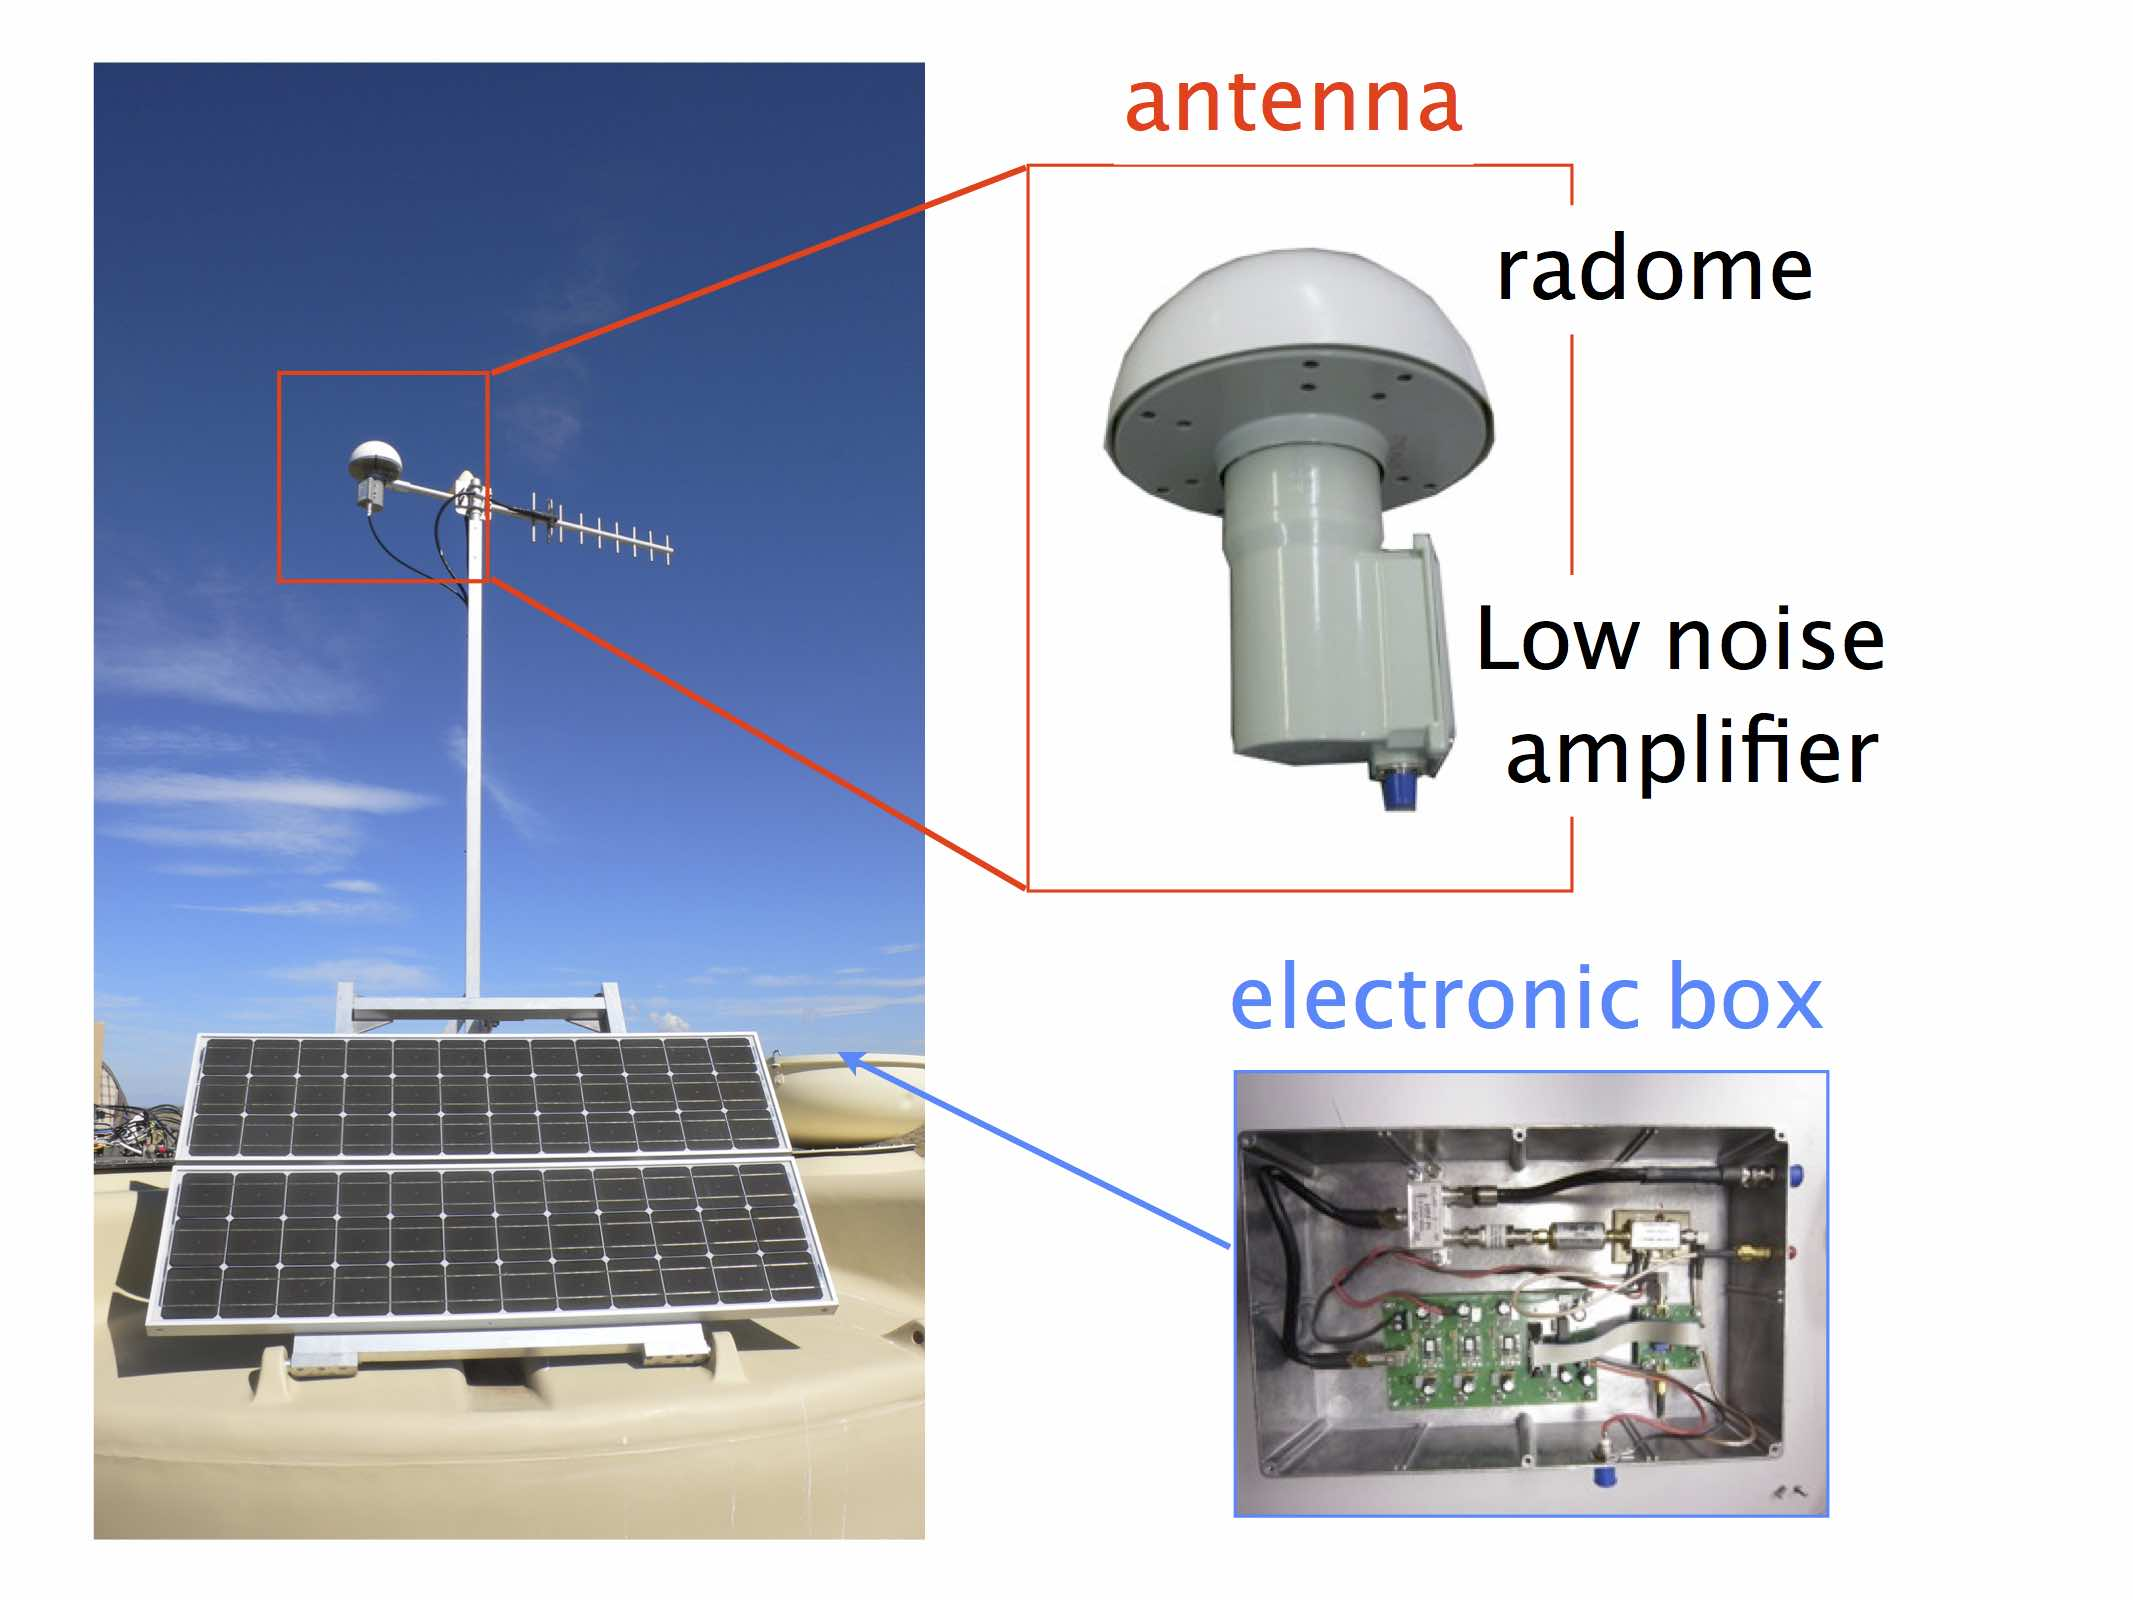
\includegraphics[width=0.49\linewidth]{setupGHznew.jpg}}
  \subfigure{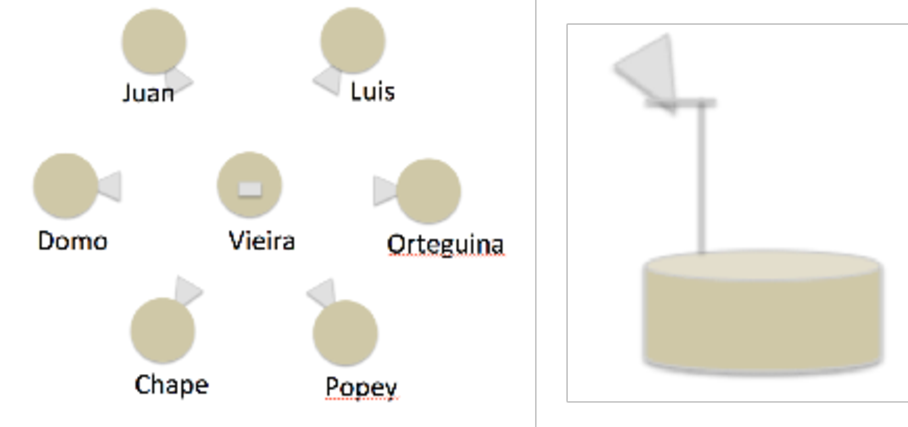
\includegraphics[width=0.49\linewidth]{GD.pdf}}
  \caption{Left: EASIER  detector installed on a  Pierre Auger surface
    detector. Right: Top  view of GIGADuck array  and side view  of one of
    the detector.}
  \label{fig:detector}  
\end{figure}

\subsubsection*{GIGADuck}
A recent calculation  of the MBR signal pointed  out that the expected
signal should  be lower by two orders of  magnitude than the
first estimation presented in~\cite{Gorham}. This consideration led to
the  design  and  the  installation  in March  2015  of  GIGADuck,  an
optimized array  of seven detectors with  a higher gain  antenna and a
different  geometry.   A pyramidal horn of 15dB  gain  antenna from A-Info company increases the  maximum antenna effective area by a factor six with respect to EASIER61.  Furthermore, the array is now composed of a central detector pointing to the zenith and the six peripheral detectors are tilted by 20$\rm ^{\circ} $ in zenith and have their azimuth adjusted to point towards the central detector as represented on the scheme of the Fig.~\ref{fig:GD}.  This configuration  increases the overlap of the detectors' field of view and enhance the probability to obtain a coincident detection. This configuration was chosen because the observation of a coincidence between two radio detectors would support the hypothesis of an isotropic emission.\\
%The  optimized  tilt angle  was  found  as  a compromise  between  the coincidence  probability  and the  antenna  temperature increase  (the brightness temperature  of the sky  increases with the  zenith angle).
As an example of the improved performance of GIGADuck, we show the simulation of the MBR of a vertical 10 EeV shower collected with  an EASIER and a GIGADuck antenna at a distance of  \unit[750]{m}. In this particular case, the ratio between GD and EASIER is around 2 for the vertical and around 10 for the tilted GIGADuck antenna. These differences is the combination of a higher of GIGADuck antenna (illustrated by the vertical antenna comparison) and the part of the shower pointed by the main lobe (illustrated by the large improvement of the inclined case). Further comparison of their performances are given in section~\ref{simulation}.

\begin{figure}[!ht]
  \centering
  \hspace*{-3ex}  
  \subfigure{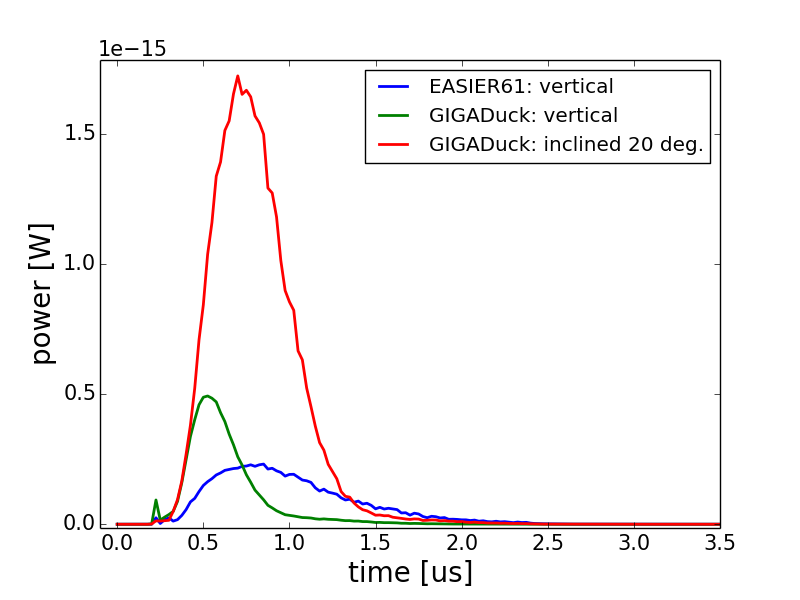
\includegraphics[width=0.49\linewidth]{EAGDexample.png}}
  \caption{Left: Top  view of GIGADuck array  and side view  of one of
    the detector.   Right: Maximum power  received from a  vertical 10
    EeV shower as  a function of its core distance  from an antenna in
    an EASIER-like configuration and a GIGADuck configuration.}
  \label{fig:GD}  
\end{figure}

\section{Detector calibration}
\label{sec:calibration}	
EASIER detectors  are required to measure faint  and impulsive signal.
A figure  of merit  of the  sensitivity used in  the field  is usually
given by:
\begin{equation}
\rm  F  =  \frac{k_{B}\cdot  T_{sys} }{A_{eff}\cdot  \sqrt{\Delta  \nu
    \Delta t}}
\label{eq:sensitivity}  
\end{equation}
F  represents the  flux  from a  signal  that would  equate the  noise
fluctuation;  $\rm T_{sys}$  is  the noise  system temperature, it is the sum of the thermal noise collected by the antenna and the electronics noise  added mainly by the first amplifier; $k_B$ is  the Boltzmann constant;  the square  root term is the amount of samples  over which this noise is  averaged, in simple case
it is the product of the  bandwidth $\Delta f$ with a time constant of
a low pass filter but in the  case of transient signal, it is meaningful
to use the expected duration of the signal. Finally, $\rm A_{eff}$ is
the effective  area of the antenna  i.e.  the portion  of the incoming
radio flux transformed into electrical power.
\subsection{sensor calibration}
%The   sensor,  the   antenna  and   the  LNB,   will   participate  in
%eq.~\ref{eq:sensitivity}  in   most  of   the  term.
\paragraph{antenna effective area}
The effective area is derived from the knowledge of the antenna gain pattern, i.e. the gain of the antenna as a
function of the direction.
Indeed, the effective area for a particular wavelength $\lambda$, in  a given direction $\theta, \phi $ can be expressed as:
\begin{eqnarray} \label{aeff}
\rm A_{eff} (\theta, \phi) = {{\lambda^2\ G(\theta, \phi)}\over{4 \pi} } 
\end{eqnarray}
The gain pattern can be either measured or simulated. 
 It has been measured for the antenna DMX241 from WS International (Fig.~\ref{fig:wsi-imep}-top),  and for an ATM horn coupled to a LNB Norsat
  in an anechoic chamber at the IMEP (Institut de
Microelectronique Electromagnetique et Photonique) at
Grenoble. The angular dependence of the effective area is illustrated  in Fig.~\ref{fig:wsi-imep}-bottom.
\begin{figure}[ht]
\centering
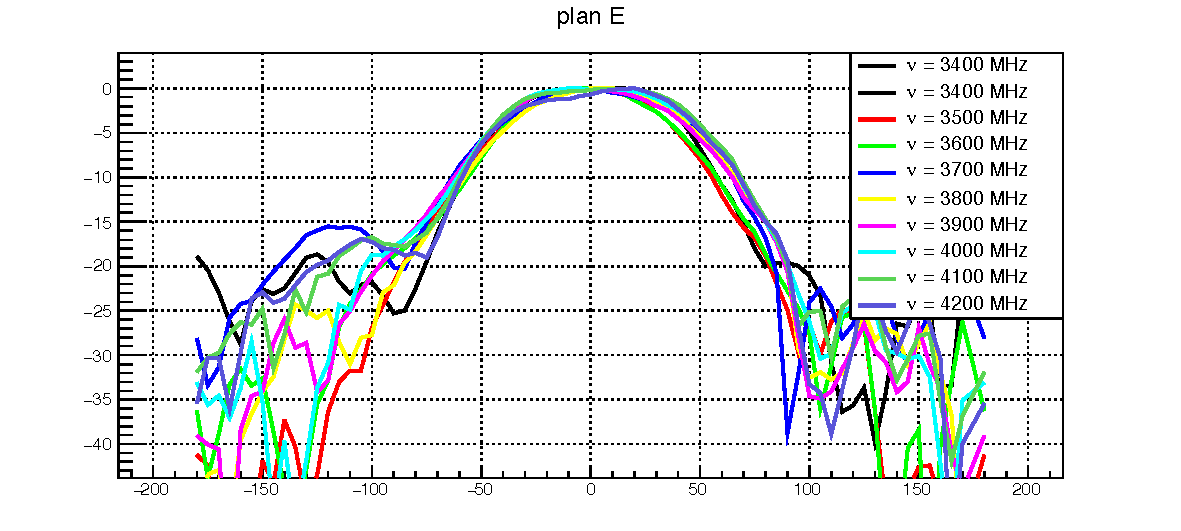
\includegraphics[width=0.49\linewidth]{../plots/C_wsi_g_E.pdf}
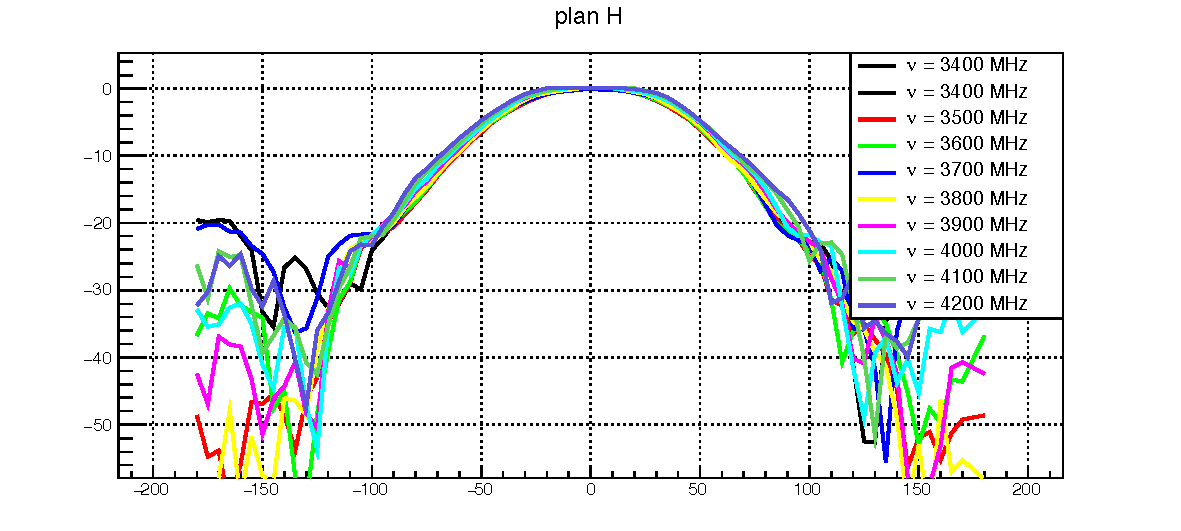
\includegraphics[width=0.49\linewidth]{../plots/C_wsi_g_H.pdf}\\
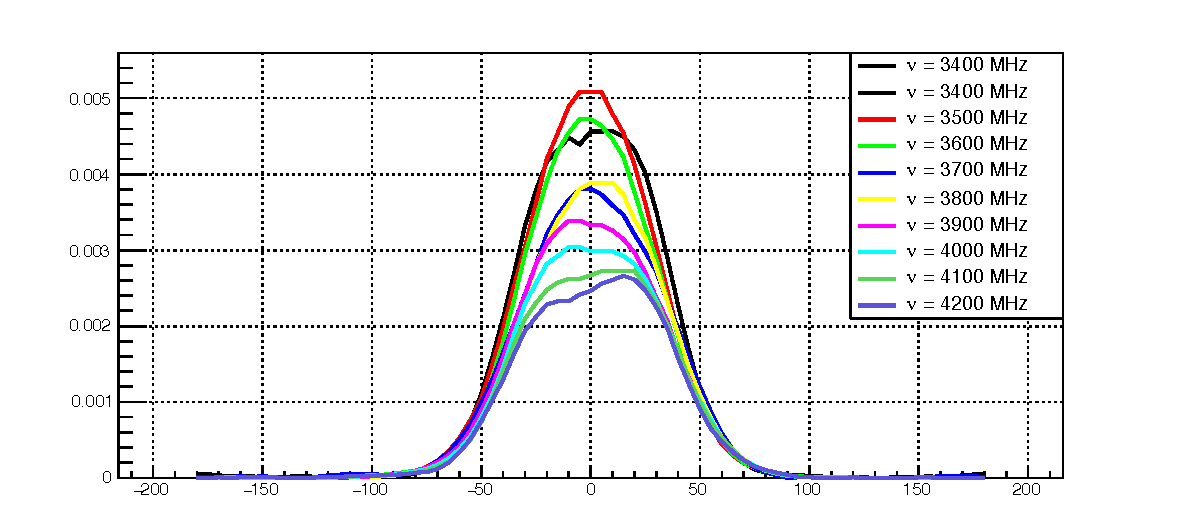
\includegraphics[width=0.55\linewidth]{../plots/C_wsi_A_EH.pdf}\\
\caption{Top: gain measurements in H and E planes- Bottom : corresponding effective area}
\label{fig:wsi-imep}
\end{figure}  
 In addition to these measurements, 
the High Frequency Simulation Software (HFSS) from ANSYS was used to simulate the
patterns of the different tested antenna types, taking into account the setup of the sensors, such as the presence of a radome.
% It  allows modeling the effect of the ground, water tank and all the surroundings on the antenna pattern.
Two different pyramidal horns (ATM and A-INFO) with 15~dB gain were simulated using HFSS~\cite{HFSS} to retrieve their gain patterns with the same free space conditions, at 3.8 GHz (Fig.~\ref{fig:A-INFO_radome}). Gain and beamwidth values from the simulation results are found to be compatible with the spreadsheets.
% as shown  in Table ~\ref{tab:pyramidal-horns}. 
A compromise between the expected performances and the cost led to the selection of seven A-INFO type horns.

\begin{figure}[ht]
\centering
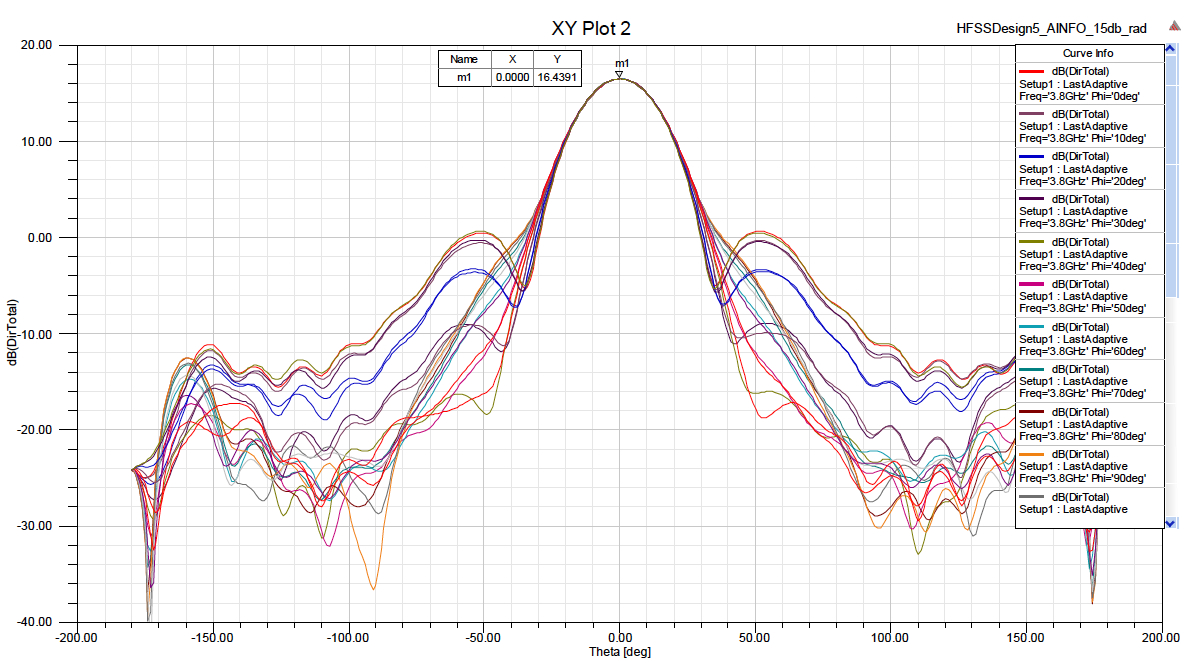
\includegraphics[width=0.5\textwidth]{../plots/AINFO_15dB_radome_pattern_HFSS.jpg}
\caption{\small{A-Info diagram with radome}}
\label{fig:A-INFO_radome}
\end{figure}  
A radome consisting of a plexiglas slab had to be fixed on the horn aperture to shield the antenna against UV, humidity. The attenuation effect of this plexiglas slab (2~mm thick, protected against UV) was evaluated using HFSS : the loss $L$ is found to be 0.17~dB. The power loss measured in the half spherical radome used for the standard EASIER61 antennas gives 0.5 dB ($\sim$31 K), more important than found for these new antennas.


%\paragraph{antenna temperature}
%The system temperature makes use of the effective area...
\subsubsection{system noise temperature}
%The noise in the EASIER and GIGADuck radio system is the sum of the antenna temperature estimated according the Eq~\eqref{tant} and the electronics noise  temperature which main contributor is the first amplifier.
%arise from on one side the thermal noise of the surrounding material collected by the antenna lobe, the antenna temperature $\rm T_{ant}$ and on the other side the electronics noise $\rm T_{elec}$.  It is  related to  the system power $\rm P_{sys}$ through:
%\begin{equation}
%  \rm  P_{sys}  =  k_{B} T_{sys}  G  \Delta  \nu  = k_{B}  (T_{ant}  +
%  T_{elec}) G \Delta \nu
%\end{equation}
%with G the electronics gain and $\rm \Delta  \nu$ the bandwidth.  The system temperature of a device is measured by comparing the output of the device when two different sources of noise are applied to its input. This method permits to cancel out the gain term in the calibration equation. A common method is to make use of an astronomical source with an known flux as a calibration source. This method is suitable when the flux is intense enough to be observed in the device. We used the sun as a calibration source to calibrate the GIGADuck detectors, see section~\ref{sec:gdtsys}. For EASIER detector and their smaller gain antenna, this method couldn't be used. Instead we setup a simple experiment consisting of the comparison of the signal when the antenna look down to the ground and when it looks up in the sky.
\paragraph{EASIER61}
The method implemented to measure the electronics noise temperature of the EASIER61 detectors relies on the so called Y-factor method. It extracts the noise temperature of a device, here the EASIER61 electronics, with the measurement of two different input noise powers. In the case of EASIER61 we simply pointed the antenna toward the ground and then toward the sky so that the electronics is subjected to two different antenna temperature. Then the temperature is found with the following equation:
\begin{equation}
	\rm	T_{elec} = \frac{T_{hot} - YT_{cold}}{Y-1} \ where \ Y = \frac{P_{hot}}{P_{cold}}
\end{equation}
where $\rm T_{hot}$ ( $\rm T_{cold}$ ) is the antenna temperature when the antenna points toward the ground (the sky) and $\rm P_{hot}$ ($\rm P_{cold}$) are the corresponding powers. The antenna temperatures are computed according:
\begin{equation}
\rm  T_{ant} = \rm \int_{\theta =  0}^{\theta = \pi}\int_{\phi = 0}^{\phi =
    2\pi} T_{B}(\theta) G(\theta,\phi) \sin(\theta) d\theta d\phi
\label{eq:tant}
\end{equation}
with $\rm T_{B}(\theta)$ the brightness temperature, around \unit[4]{K} for the sky at the zenith and \unit[270]{K} for the ground. Antenna temperatures if  $\rm T_{hot} = \unit[260]{K}$ and $\rm T_{cold} = \unit[6]{K}$ are obtain. \\ The measurement took place in the pampa at the detector's site. The setup comprises the main component of the installed detectors namely the LNBf, the radome and the power detector Minicircuit ZX47-50. The antenna was oriented consecutively up and down and the voltage of the power detector was recorded with a portable oscilloscope. The voltage difference between the two measurement is related to a difference of power according the calibration curve  of the power detector (see section~\ref{sec:calibration}). For the two types of LNBf used in EASIER61, we found system noise temperatures of $\rm T^{GSI}_{elec} =  \unit[114]{K} \pm 10$ and $\rm  T^{DMX}_{elec}  =  \unit[97]{K}   \pm  9$. The errors include an uncertainty on the calibration factor in Eq.~\eqref{eq:delvdelp} of 1mV/dB and a spread of the ground brightness temperature of $\rm \pm \unit[10]{K}$ due to the poorly known physical temperature and emissivity.


%Because the measurement of the gain with a high precision is hard to achieve, the main method to retrieve the system
%temperature  is to  combine two  measurements with  a  different input
%noise power -  or the equivalent temperature - to  cancel out the gain
%term.  The  system noise temperature  of EASIER and GIGAS's  LNBf were
%measured by  the CROME collaboration  comparing the output  power when
%the  antenna collects noise  from surrounding  material first  at room
%temperature       and        then       at       liquid       nitrogen
%temperature~\cite{bib:gapnoteCROME}.   The electronics  temperature of
%the GI 301 was  found to be very variable from 40  to 180K, the one of
%the WS  International stable  at 25K and  the Norsat at  23.5K.  MIDAS
%experiment  uses  also  the  LNBf  WSI DMX241  and  measured  a  noise
%temperature  of  25K~\cite{bib:midas}.   We  have  also  measured  the
%electronics noise temperature of  the WSI DMX241 comparing the spectra
%measured at room temperature in  laboratory when the antenna is facing
%an absorber ($\rm T_{room} = \unit[300]{K}$) with the measurement when
%the  antenna faces  the  sky ($T_{sky}  = \unit[7]{K}$).   \textit{The
%  results   we  obtain  for   amounts  to   around  $\rm   T_{elec}  =
%  \unit[40]{K}$.     The   difference   with    previously   mentioned
%  measurements can  be explained  by the radome  protection.}
\paragraph{GIGADuck}
For the GIGADuck antennas, since their gain is larger, the sun passage is observed in the monitoring data and can be used as a calibration source.  The increase  of power induced upon the passage of the sun in the antenna field of view reads:
\begin{equation}
  \rm       \unit[\Delta      P]{[dBm]}       =       10      log_{10}
  (\frac{P_{sys} + P_{sun}(\theta_{sun},\phi_{sun})  }{P_{sys}} )  = 10
  log_{10}     (    1     +     \frac{    \frac{1}{2}F_{sun}     \cdot
    A_{eff}(\theta_{sun},\phi_{sun}) } {T_{sys}} )
  \label{eq:deltaP}
\end{equation}
where    $\rm   F_{sun}$    is    the   total    solar   flux which is measured by dedicated solar observatory like~\cite{sundata} or~\cite{nobeyama},    $\rm A_{eff}(\theta_{sun},\phi_{sun}) $ is the antenna effective area for the given position of the sun in  the sky and the factor $\rm \frac{1}{2}$ is  the polarization factor.  This measurement can be performed only when the sun is  in the field  of view of  the antenna. As  it is shown  in the
Fig.~\ref{fig:sunsim} (left), the sun  is not visible by any antenna of the  GIGADuck array  during austral winter  but will cross  the field of view of five of them during summer.\\ We  retrieve the absolute value of  the daily average sun    flux   at   \unit[2.8]{GHz}    measured at the Dominion Radio Astrophysical Observatory and publicly released at~\cite{sundata}.  The  flux at the  center frequency of  the C-band, \unit[3.8]{GHz},   is  obtained   by   using  parameterization   found in~\cite{sunparam, sunparam2}. 
\begin{figure}[!ht]
 \centering
 \hspace*{-3ex}
 \subfigure{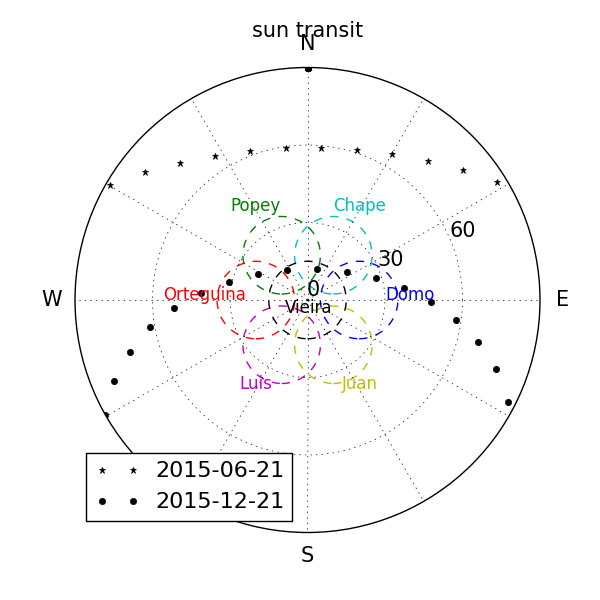
\includegraphics[width=0.39\linewidth]{sunpolar.png}}
 \subfigure{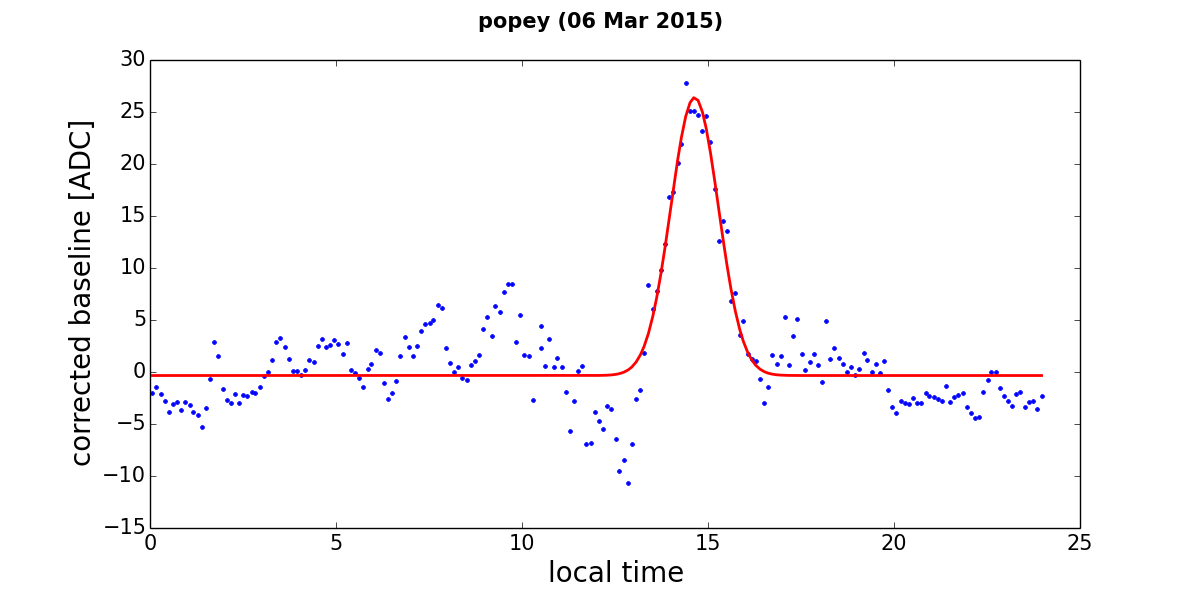
\includegraphics[width=0.6\linewidth]{fitexample.png}}
%% \subfigure{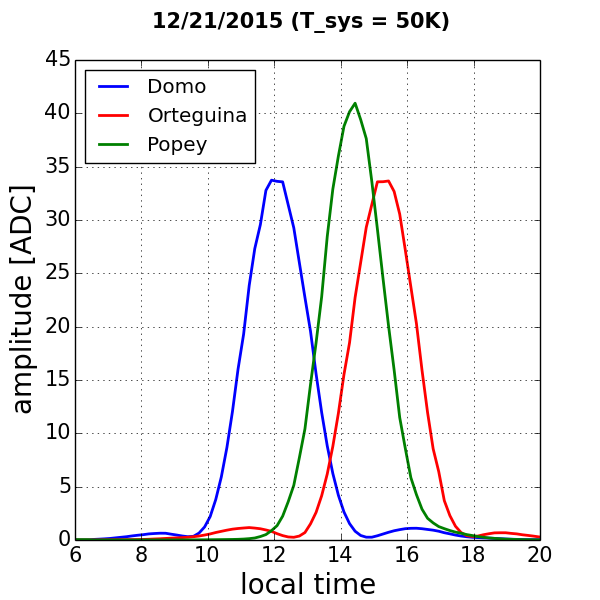
\includegraphics[width=0.49\linewidth]{sunexpected.png}}
 \caption{Left: Sun transit for the two solstices. The colored circles
   represent  the field  of  view of  the  GIGADuck antennas.   Right:
   Example  of the  baseline during  one  day. In  blue is  the
   orignal baseline when the mean is subtracted, in green after it was
   corrected from temperature dependence and  in red is a gaussian fit
   of to extract the signal from the sun.}
%%    Simulated  baseline  increase for  three  antennas  during the  sun
%%    passage.}
 \label{fig:sunsim}
\end{figure}
Since GIGADuck data are  part of  the SD  data stream  including the monitoring system, the radio  baseline is recorded every \unit[400]{s} with other  information such as  the outside temperature. The sun signal is extracted from these data with the following method.  First the rainy periods are removed, since rain and  high humidity  affect the radio  baseline in a non trivial way. Then this data set is used to correct for a linear  dependence of the system's gain with the outside temperature (the time when the sun is expected is removed for this parameterization). The final step consist in fitting the bump induced by the sun flux with a Gaussian function. The maximum of the fitted function is then converted in power difference according Eq.~\eqref{eq:eqcalibration} and the system noise temperature is retrieved with Eq.~\eqref{eq:deltaP}.\\ This method was applied for four antennas and the results for each day for two of them are shown in the Fig.~\ref{fig:GDtempres}. Some measurements show a large error bar due to the uncertainty on the value of the maximum of the baseline that particular day. The obtained temperature are \unit[39, 45, 59 and 70]{K}. The system noise temperature of the three other detectors are taken as the maximum measured to remain conservative.

\begin{figure}[!ht]
 \centering
 \hspace*{-3ex}
 \subfigure{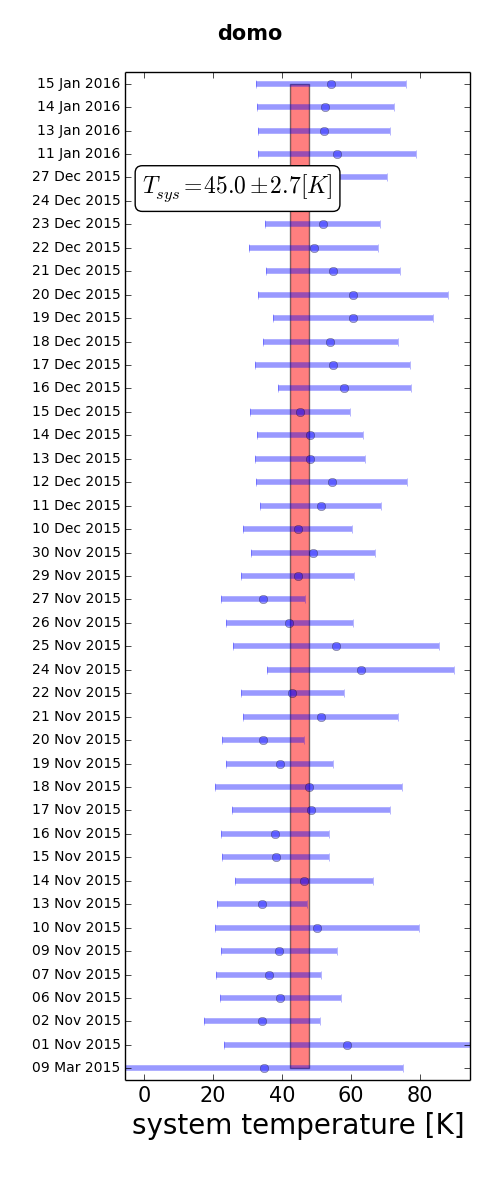
\includegraphics[width=0.25\linewidth]{domosystemp.png}}
  \subfigure{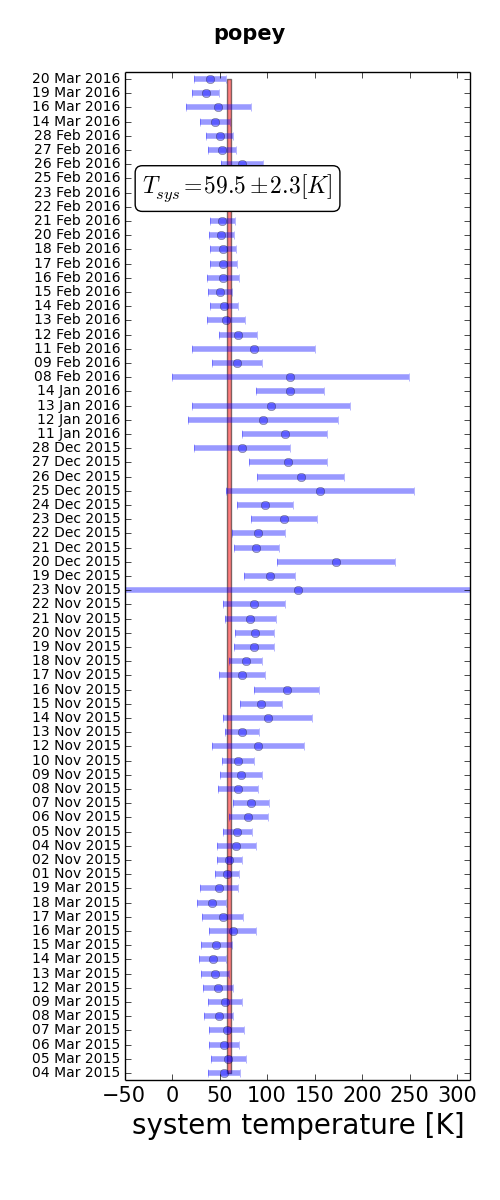
\includegraphics[width=0.25\linewidth]{popeysystemp.png}}
  \caption{Temperature measured for two GIGADuck detectors with the sun signal.}
 \label{fig:GDtempres}
\end{figure}


\paragraph{sensor bandwidth}
The absolute gain  of the RF part which includes the amplifier the bias tee, the cables etc, does  not  enter  directly in  the  detector's sensitivity,     but    the     frequency    bandwidth     does    (cf eq.~\ref{eq:sensitivity}).  The  normalized gain  of the LNB  used for EASIER61 (GI301, DMX241) and GIGADuck (Norsat 8115) are represented in the  Fig.~\ref{fig:normalizedgain}  and  the  effective  bandwidth  is computed according:
\begin{equation}
  \rm \Delta \nu = \frac{1}{G_{max}} \int G(f) \cdot df
\end{equation}
We  obtain effective bandwidths  of \unit[437  $\rm \pm$  30]{MHz} and
\unit[445 $\rm \pm$ 56]{MHz} for the GI301 and the DMX241 respectively
and \unit[750]{MHz} for the Norsat.
\begin{figure}[!ht]
  \centering
  \hspace*{-3ex}
 \subfigure{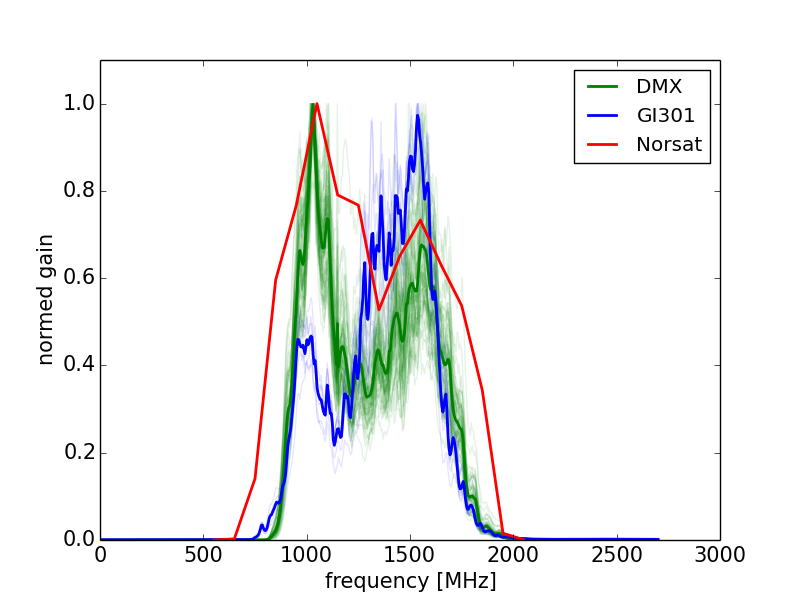
\includegraphics[width=0.49\linewidth]{spectra3.png}}
  \caption{Normalized  gain  of the  three  mentioned  LNBf after  the
    frequency downconversion.  The thick blue and green  lines are the
    average over several detectors. Only one measurement was performed
    with the Norsat LNBf (in red). }
  \label{fig:normalizedgain}
\end{figure}


\subsection{Adaptation electronics calibration}
\label{sec:elec}
\subsubsection{Specification}
The adaptation electronics is composed of the power detector, the adaptation board and ends the analog to digital converter of the Auger SD.  The power detector is an Analog Device AD8318 (in the encapsuled version Minicircuits ZX47-50), it is  a logarithmic  amplifier with a  wide bandwith and  large power
dynamic  range.  For the first seven detectors its output  voltage  was  filtered  with  an  output capacitor  but this capacitor is removed for  the  following version   EASIER61  and  GIGADuck.  The power detector output voltage $\rm V_{pd}$ was calibrated in laboratory using a noise waveform at various power $P_{in}$ as input:
\begin{equation}
  \rm  V_{pd} [V] =  -0.0234\cdot P_{in} [dBm] + offset
\label{eq:eqpd}
\end{equation}
 The  power detector  voltage is  then amplified  by a  factor  4.2 to
 obtain  a final  power dynamics  of \unit[20]{dB}  over the  1024 ADC
 counts of the  SD acquisition. The overall conversion  from the input
 power to the ADC is:
\begin{equation}
  \rm ADC = 50.2\cdot P [dBm] + offset
\label{eq:eqcalibration}
\end{equation}
An offset was designed to be adjustable to make up for the differences of the detectors gain.

\subsubsection{Time response and electronics simulation}
In  the  following  paragraphs  we  study the  time  response  of  the
adaptation  electronics. 
\paragraph{power detector}
To understand the power detector response to impulsive signals, we set  a detection chain in laboratory composed  of a LNBf  followed by a  power detector. A fast oscilloscope is  used to record simultaneously the  LNBf and power
detector's  output. We  used the  spark  of an  electronic lighter  to
produce a short and broadband  signal and emulate  the signal from an  air shower. An example of these signal is shown in the Fig.~\ref{fig:powerdetsim}. We  find that the power detector output is well reproduced when one perform  a convolution of the input signal in dBm (logarithmic unit) and an exponential function with a decay constant $\rm \tau$:
\begin{equation}
  \rm V_{PD}(t) = k_{1}\cdot \int_{t>0}P_{dBm}(u)exp(\frac{t-u}{\tau})du + k_{2}
  \label{eq:convolution}
\end{equation}
The factor    $\rm   k_{1}$  is fixed to   the   conversion    factor   of   the
equation~\ref{eq:eqpd} and $\rm   k_{2}$ is an offset. We simulate fake waveforms from measured RF signal with various decay times  $\rm \tau$. The best $\rm \tau$ is found by minimizing the distance $\rm d = \Sigma (V_{measured} - V_{simulated})^2$ between simulated and measured power detector waveforms.  We found $\rm \tau_{capa}  = \unit[41.5]{ns}$ when an  output capacitor follows the power detector and $\rm \tau_{nocapa} = \unit[6.3]{ns}$ without. 
\begin{figure}[!ht]
 \centering
 \hspace*{-3ex}
 \subfigure{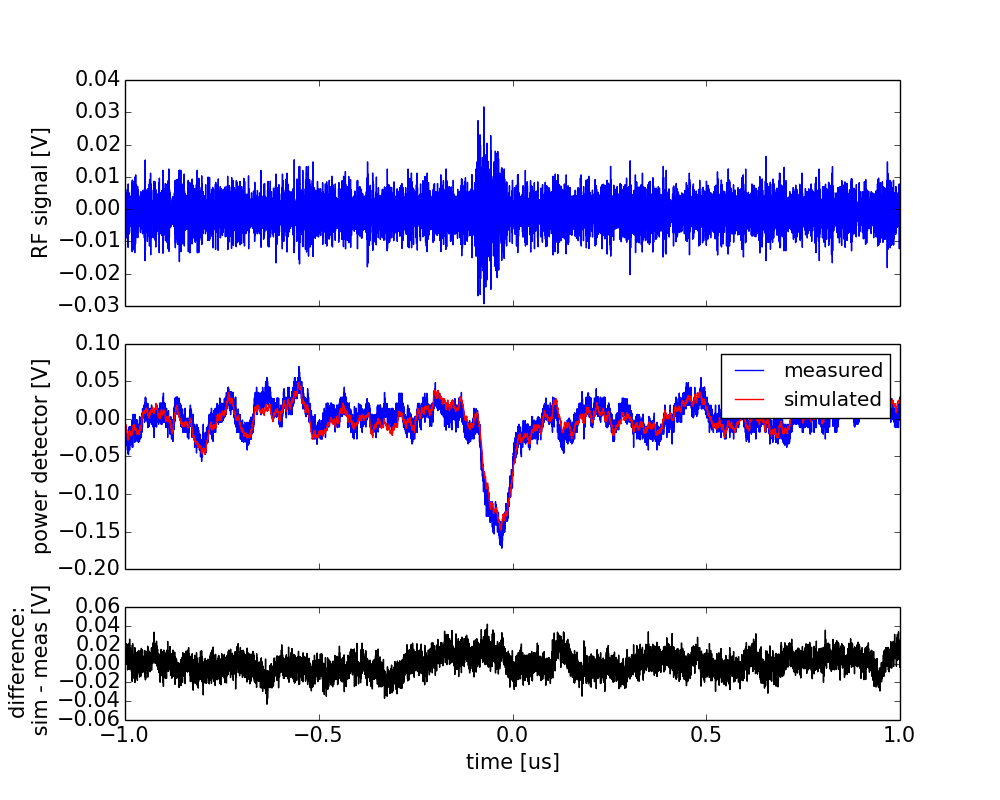
\includegraphics[width=0.7\linewidth]{capa_method3.png}}
 \caption{Example  of RF  and power  detector waveforms.  The measured
   waveforms are in blue and the simulated one in red. The lower panel
   show the difference.}
 \label{fig:powerdetsim}
\end{figure}
\paragraph{Adaptation board}
To measure the response of  the adaptation board, we add it to the calibration setup described in the previous paragraph.  We  recorded simultaneously the  input of the  board and  its  output. We  find the  board's response  by measuring the its transfer function in the frequency domain:
\begin{equation}
  \rm \tilde{H}(f) = \frac{\tilde{V}_{out}(f)}{\tilde{V}_{in}(f)}
\end{equation}
The  gain and the phase of the board is  represented  in  the  Fig.~\ref{fig:board}. \\The last part of  the chain, the Auger front  end is simulated with  a low pass filter with $\rm f_{cut} = \unit[20]{MHz}$ and by sampling in time and amplitude.
\begin{figure}[!ht]
 \centering
 \hspace*{-3ex}
 \subfigure{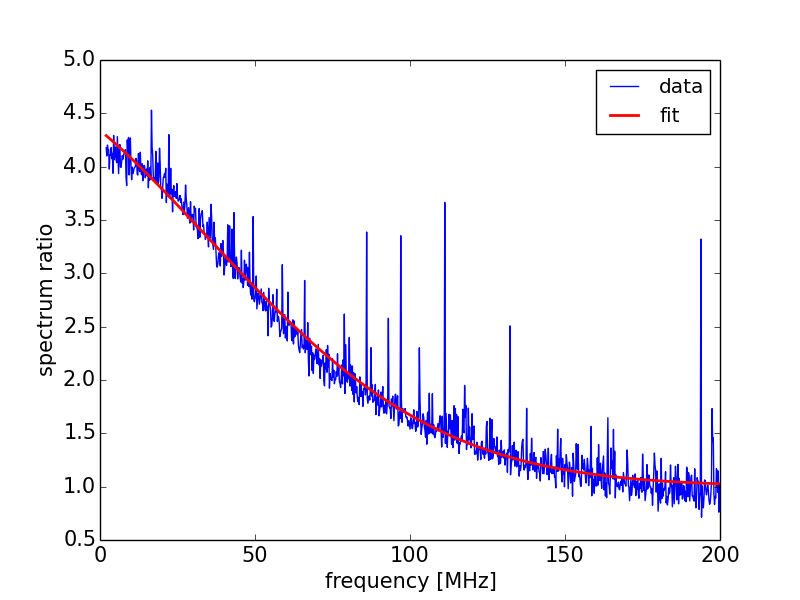
\includegraphics[width=0.49\linewidth]{fitspecboard2.png}}
 \subfigure{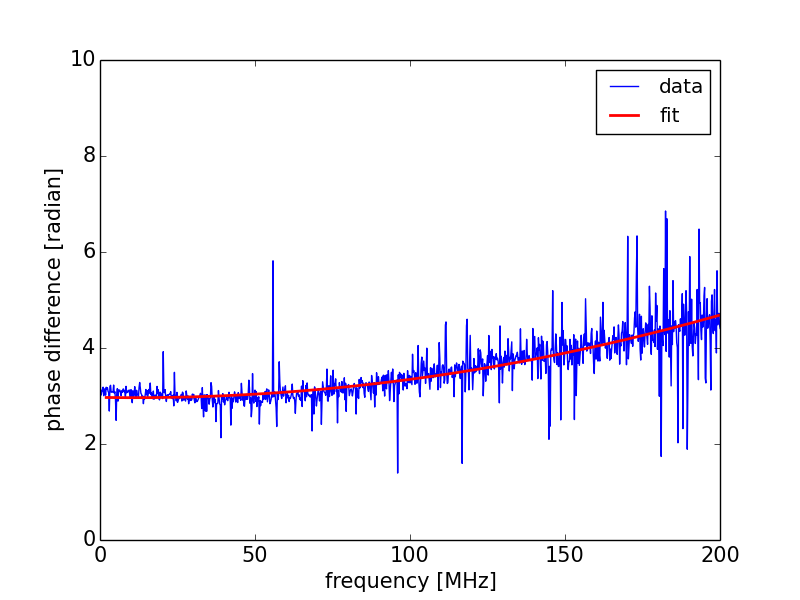
\includegraphics[width=0.49\linewidth]{fitphaseboard.png}}
 \caption{Measurement and fit of the gain and phase of the adaptation board.}
 \label{fig:board}
\end{figure}

\paragraph{validation with data}
In order to  validate the calibration and simulation,  we produced some mock data   
and compare them with the  actual radio waveform  we record in  the Auger data.   An RF waveform   is  generated   from   the  spectra   represented  in   the Fig.~\ref{fig:normalizedgain}   by  inverse  FFT.    The  adaptation electronics simulation  is then applied to  it in order  to produce an trace    in   ADC    count.     The Fig.~\ref{fig:distcomparison} the distribution  of the noise for the
data (in grey)  and the simulation (in red).  The comparison are shown
for the three setups.
\begin{figure}[!ht]
 \centering
 \hspace*{-3ex}
 \subfigure{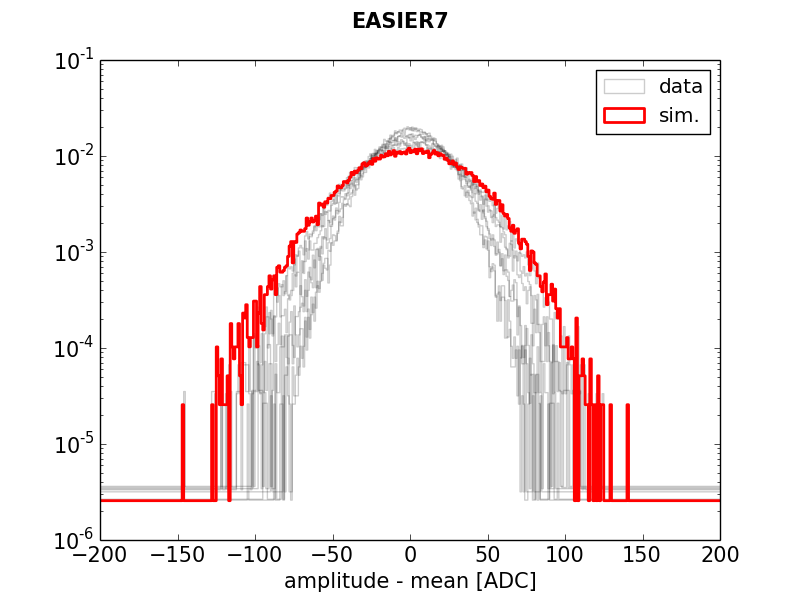
\includegraphics[width=0.32\linewidth]{m3_distdatasimEA7.png}}
 \subfigure{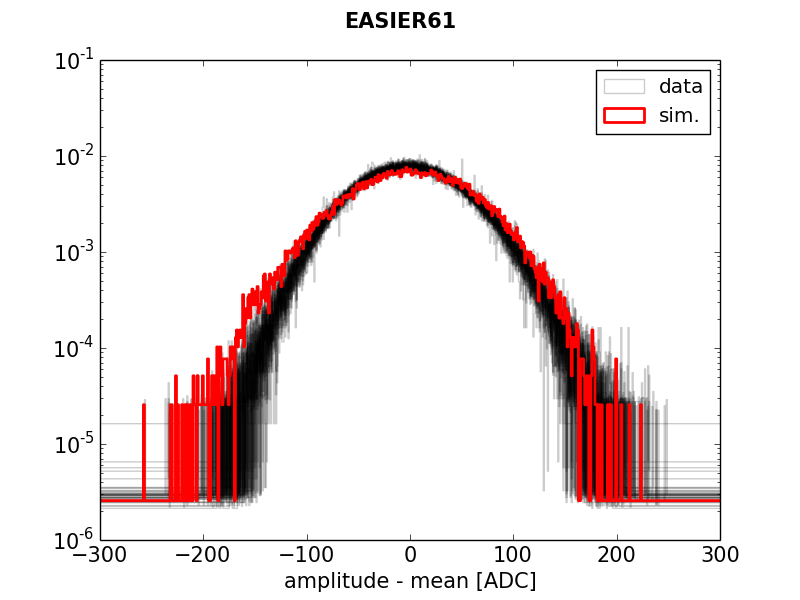
\includegraphics[width=0.32\linewidth]{m3_distdatasimEA61.png}}
 \subfigure{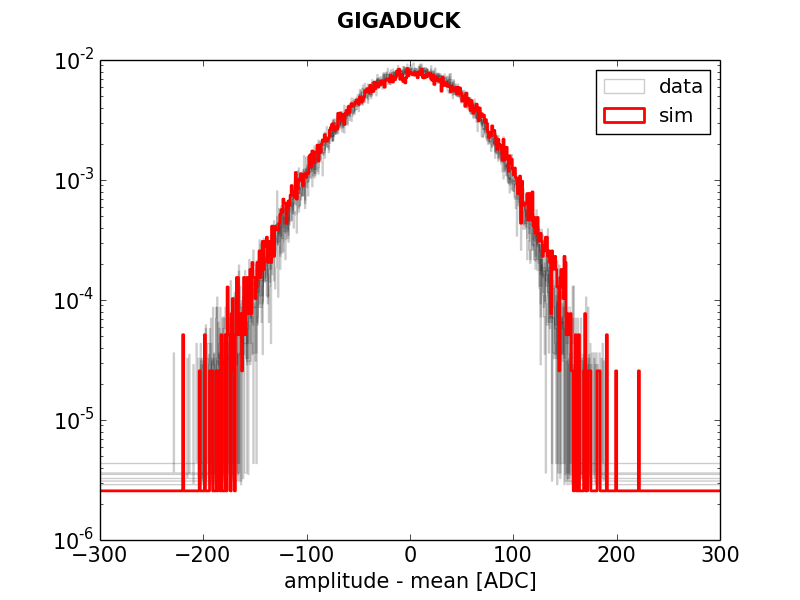
\includegraphics[width=0.32\linewidth]{m3_distdatasimGD.png}}
 \caption{Distribution of the waveform value for simulated and measured data for the EASIER61 setups (left and middle) and for the GIGADuck setup (right)}
 \label{fig:distcomparison}
\end{figure}
If the simulations agree very well for EASIER61 and GIGADuck, it tends
to overestimate the noise fluctuation for the first setup. However the
measured and simulated standard  deviation of the distributions differ
 at maximum by 15 ADC counts which represent \unit[0.3]{dB} or 7\%.


\section{Expected sensitivity}
\label{simulation}
 \subsection {End-to-end MBR simulation }
  %%%%%%%%%%%%%%%%%%%%%%%%%%%%%%%%%%%%%%%%%%%%%%%%%%%%%%%%%%%%%%%%%%%%%%%%%%%%%%%%%%%%%%%%%%%%%%%%%%%%%%%%%%%%%%%%%%%%%%%%%%%%%%%
  	Simulation of the emitted MBR is based on the model elaborated in~\cite{ALSAMARAI}. In this section, the simulation of the shower as well as the MBR emission and the propagation of the radiation until the detectors are presented. 
  \subsection { MBR emission simulation }
  %%%%%%%%%%%%%%%%%%%%%%%%%%%%%%%%%%%%%%%%%%%%%%%%%%%%%%%%%%%%%%%%%%%%%%%%%%%%%%%%%%%%%%%%%%%%%%%%%%%%%%%%%%%%%%%%%%%%%%%%%%%%%%%
 In order to perform a fast simulation, a Gaisser-Hillas parametrization of longitudinal profiles of air showers was used as in \cite{PERRONE}. The number of charged particles at a certain depth $X$ can be retrieved from the following expression: 
      	\begin{equation}
  	N (X-X_1) =   N_{\mathrm{max}} \left(\frac{X-X_0}{X_{\mathrm{max}}-X_0}\right)^{\frac{X_{\mathrm{max}}-X_0}{\lambda}} \exp{\left(\frac{X_{\mathrm{max}}-X}{\lambda}\right)}, 
 	\end{equation}
	where $X_1$ is the physical depth of the first interaction point, $N_{\mathrm{max}}$ is the maximum number of shower particles, and X$_{\mathrm{max}}$ is the atmospheric depth at shower maximum in g~cm$^{-2}$.
Tabulated mean and RMS values of Gaisser-Hillas parameters for proton primaries were retrieved for different energies in $\log_{10}$($E$/eV) = [17.5, 21.0]. A linear interpolation in $\log_{10}$($E$/eV) provides the relevant parameters to be used as input values at any energy. For the parameters $X_0$, $N_{\mathrm{max}}$, $X_{\mathrm{max}}$, $\lambda$, randomization is performed using a gaussian distribution while for $X_1$, an exponential distribution is used.
The energy of the shower is generated randomly following the energy spectrum in the region above the ankle, between 4$\times$10$^{18}$~eV and 3$\times$10$^{20}$~eV using a power law function as defined in~\cite{SCHULZ}: 
	\begin{equation}
	J(E; E > E_a) \frac{ E^{-\gamma_2} } {1+ \exp \left({ \frac{\log_{10}E - \log_{10}E_{1/2}}{\log_{10}W_c} }\right)},
	\end{equation}
	where the spectral index above the ankle $\gamma_2$ is 2.63. The term $\log_{10}E_{1/2}$ is the energy at which the flux has dropped to half of its peak value before suppression, and $\log_{10}W_c$, is its associated steepness, they are fixed to 19.63  and 0.15 respectively. 
	
	Shower cores are generated randomly inside a hexagon representing the fiducial area of a hexagonal array of 7 antennas. The axis of the shower is defined as random in azimuth $\phi$ and random in the cosine of the zenith $\theta$ limited to 60$^\circ$. 
	Starting from the first interaction point high in the atmosphere, the number of primary electrons is calculated in grammage steps of $dX$ = 2.5 g~cm$^{-2}$ until it reaches the height level of the antenna. At each step, the mean energy deposit per particle E$_{\mathrm{dep}}$ is calculated following CORSIKA parameterization at 1 MeV as given in~\cite{NERLING}. 
	
	Assuming that ionization is the main process that these electrons undergo, the number of the resulting secondary electrons at each step in $X$ is calculated as:
	\begin{equation}
	N_{\mathrm{ioniz}} = \frac{E_{\mathrm{dep}}(X)~\rho(a(X,\theta))}{I_0 + \left\langle T_e \right\rangle},
	\end{equation}
	where $\rho(a(X,\theta))$ is the atmospheric density at a certain height in the atmosphere, and $I_0$ is the ionization potential (equivalent to 15.6~eV for N$_2$ and 12.1~eV for O$_2$ molecules). $\left\langle T_e \right\rangle$ stands for the mean kinetic energy of the secondary electrons, equivalent to 40~eV, as found in~\cite{ALSAMARAI}. At each step of the development of the shower in altitude, and for each emitter comprised in a thin disk of height d$a$ being within the Moli�re radius of the shower, the microwave power is: 
	\begin {equation}
	P_{\mathrm{MW}} = hc~\frac{N_A}{M}~\rho(a)~N^{\mathrm{tot}}_{\mathrm{ioniz}}~\tilde{\sigma}(t=0,a),
	\end{equation} 
	where $h$ is the Planck constant, $c$ is the speed of light, $N_A$ is the Avogadro number, $M$ is the dry air molar mass, and $N^{\mathrm{tot}}_{\mathrm{ioniz}}$ is the number of secondary electrons present in the thin disk of height $da$. The position of the emitter is randomly chosen in order to sample uniformly the azimuth $\psi$ around the shower axis and $r\times$ldf$(r,\psi)$, with $r$ the distance to the shower axis at the current altitude and ldf$(r,\psi)$ the NKG function. $\tilde{\sigma}(t=0,a)$ stands for the effective cross-section, proportional to the free-free interaction cross-section responsible of MBR emission. Its value is assigned to 1.7$\times$10$^{-28}$~m$^2$ at $t=0$ following the calculations found in \cite{ALSAMARAI}. Formally speaking, this cross-section is dependent on altitude. This dependence is negligible after reaching X$_{\mathrm{max}}$, thus, only a small number of interactions before X$_{\mathrm{max}}$ are neglected.
	Once the power is calculated at the emission point, one can propagate the signal down to the detector. A model of the refractive index of the atmosphere is taken into account and is represented in Fig.~\ref{refIndex}. The refractive index is almost independent from the frequency considered, and manifests a small dependence with the height of the atmosphere. It has been verified that the influence of the variable refractive index on the amplitude and shape of the received signal is negligible.  

%\begin{figure}[h]
%\center{
%\begin{minipage}[t]{0.47\linewidth}
%\includegraphics[width=\textwidth]{./Fig/section_3/refr8index.eps}
%\caption{\small{ Refractive index as a function of height. It is almost independent on frequency. Its dependence on the height is also small.}}
%\label{refIndex}
%\end{minipage}
%\hspace{0.2cm}
%\begin{minipage}[t]{0.47\linewidth}
%\includegraphics[width=\textwidth]{./Fig/section_3/lifetime.eps}
%\caption{\small{Electron lifetime as a function of height.}}
%\label{lifetime}
%\end{minipage}
%}
%\end{figure}   
%		
	The time structure of the emission from each point follows the time dependence of $\tilde{\sigma}$. Once the electron is attached, no MBR emission is anymore possible, so that the time profile is largely influenced by the attachment process to Oxygen and Nitrogen molecules. The characteristic time scale of attachment processes is shown in Figure \ref{lifetime}. However, other effects enter into the time structure of $\tilde{\sigma}$. An accurate parameterization of $\tilde{\sigma}$ turns out to be:
	\begin{equation}
	\tilde{\sigma}(t)= \mathrm{min}\left(\tilde{\sigma}_0,\frac{0.08~\tilde{\sigma}_0~(t/\mathrm{ns})^{-0.3}}{1+(t/\mathrm{ns})^{1.5}}\right).
	\end{equation}

	The received power at the detector is then calculated as: 
	\begin{equation}
	P_{\mathrm{rec}} = \frac{P_{\mathrm{MW}}}{4~\pi~R^2}~A_{\mathrm{eff}}~\Delta \nu,
	\end{equation}
	where $R$ is the distance from the emission point to the receiver, $A_{\mathrm{eff}}$ is the effective area of the antenna, and $\Delta \nu$ is the frequency bandwidth. 

	The gain pattern of any type of antenna is obtained using \textit{HFSS}~\cite{HFSS}.
	The effective area is calculated using the gain pattern of the antenna. The following expression holds for its calculation:  
	\begin{equation}
	A_{\mathrm{eff}}(\theta, \phi) = \frac{\lambda^2~G(\theta, \phi)}{4~\pi} 
	\end{equation}
	As previously mentioned, we aim at increasing the capability of the two modified antenna setups to detect MBR signals. To increase the number of showers which can be detected by the improved sensors set on one hexagon (7 stations), each peripheral antenna of the hexagon is directed towards the central antenna, which is kept vertical. It has been shown that the value of the tilt angle optimized to enhance the signal to noise ratio by being sensitive to further showers, while keeping the noise due to the ground temperature low is 20$^\circ$~\cite{Talk}.
	For each event, on each antenna, time traces of 768 bins of 25~ns bin width are then filled by the expected power calculated above, considering the propagation and the expected time evolution of the emitted MBR photons as well as the attachment process responsible of the fading of the signal.

  \subsection {Expected sensitivity}
 %%%%%%%%%%%%%%%%%%%%%%%%%%%%%%%%%%%%%%%%%%%%%%%%%%%%%%%%%%%%%%%%%%%%%%%%%%%%%%%%%%%%%%%%%%%%%%%%%%%%%%%%%%%%%%%%%%%%%%%%%%%%%%%
	Following reference \cite{ALSAMARAI_YIELD}, it is convenient to express the sensitivity to MBR in terms of the yield. The yield quantity can be introduced in the calculation of the emitted power as:
	\begin{equation}
	\frac{d^2P}{d\nu da}(a) =Y \frac{\rho^2(a) }{\rho_0 }\left\langle\frac{dE}{dX}\right\rangle 
 	\end{equation}
	The yield quantity is dimensionless, it represents the proportionality relating the energy radiated off by MBR to the deposited energy. It is thus an appropriate quantity to describe the MBR emission. In reference \cite{ALSAMARAI_YIELD}, this quantity is equivalent to 1$\times$10$^{-12}$  in the frame of the microscopic model. To probe the sensitivity of any setup to the MBR as a function of the intensity of the emission, the yield can be inserted in the expression of $P_{\mathrm{MW}}$ with the following substitution~\cite{ALSAMARAI_YIELD}: 
\begin{equation}
\frac{hcN_A\tilde{\sigma}(t=0)}{M(I_0+\left\langle T_e\right\rangle)} \rightarrow \frac{Y}{\rho_0}.
\end{equation}

	The sensitivity to a certain yield is calculated in terms of the number of expected events using a certain type of antenna. The number of expected events per year per equipped hexagon covering an area labeled $S$, is formulated as:
	\begin{equation}
	\mu(Y) = J_0\int_{>E_0}dE~f(E) \int_{\Delta \Omega}d\Omega~\cos{\theta}\int_{\Delta S}dS~\int_{\Delta T}dt~\epsilon(E,\theta,\Phi,x,y,Y),
	\end{equation}
	where $\epsilon$ is the detection efficiency depending on the yield, the position of the shower, and its incidence angle. To avoid comprehensive tabulations of the $\epsilon$ efficiency function, this expression is estimated by Monte-Carlo:
\begin{equation}
\mu(Y) \simeq \left(J_0\int_{>E_0}dE~f(E)\right)~\left(\int_{\Delta \Omega}d\Omega~\cos{\theta}\right)~\Delta S~\Delta T~\frac{1}{N_{\mathrm{sim}}} \sum_{i=1}^{N_{\mathrm{sim}}} f_i(E_i,\theta_i,\phi_i,x_i,y_i;Y),
\end{equation}
with $f_i=1$ if the signal is detectable according to some signal-to-noise criteria and $f_i=0$ otherwise. The random set of variables $\{E_i,\theta_i,\phi_i,x_i,y_i\}$  is already selected according to the measures of the integrals in front of the Monte-Carlo summation.
A Monte-Carlo simulation of 10000 proton showers within the energy band [4$\times$10$^{18}$ eV$\ -\ 3 \times$10$^{20}$ eV] randomly hitting the fiducial area of a hexagon was thus performed for a hexagon equipped with DMX antennas, \textit{A-Info} antennas, and \textit{Helix} antennas. The result is shown in figure 7, where the scanned value on the abscissa axis is the yield quantity normalized to the theoretical one. It is found that the actual configuration of the EASIER detector is unable to detect MBR as predicted by the microscopic model. The main reason is that the EASIER detector was optimized to detect a yield which is $\sim$70 times higher than the one retrieved from the model, using the scaling law from beam measurements. The two other configurations enable an enhancement by a factor $\sim$10 at 3.8 GHz and a factor $\sim$100 at 1.2 GHz.
%\begin{figure}[ht]
%\centering
%\includegraphics[width=0.6\textwidth]{./Fig/section_3/sensitivity}
%\label{fig:yieldy}
%\caption{Number of expected events using the actual antenna array (EASIER), Helix antennas array (GigaDuck-1.2 GHz), A-Info antennas array (GigaDuck -3.8 GHz) for different values of the MBR yield.}
%\end{figure}  	

	While this optimization seems promising in particular using the \emph{Helix} antennas with $\sim$ 25 events/hexagon for one year of operation ($\sim$ 5 events/hexagon for one year using A-Info), in reality, the identification of an MBR event is still delicate. In contrast to a geosynchrotron emission or an Askaryan effect, which are possible emissions that could occur at GHz frequencies, the MBR emission is isotropic. This gives the possibility to identify it by requesting that the radiation is detected at large distances. A plausible cut would be thus performed on the number of stations that detected the event. By requesting at least 2 stations spaced on the regular array (1500 m spacing), one would discard emissions arising from geosynchrotron or Askarian effects (which expected signals expand over few hundred meters). Using the most sensitive antenna (\textit{Helix} at 1.2 GHz), the number of events after a cut on the SNR and the number of stations (quoted as channels in the figure) is shown in Fig.~\ref{fig:yildnormal}, in the case of the strict expectations from the microscopic model ($Y$=1) (left panel), and a yield value ten times higher than our calculations (right panel). Relying on the strict expectations from the microscopic model, and requesting that at least 2 antennas were sensitive to the signal using a loose cut on SNR (SNR>2), the new apparatus would be sensitive to only few events/hexagon in one year. Using the C-band antennas with this set of cuts, no events are expected. Thus, it seems very unlikely that an MBR event would be detected by more than one antenna due to the  faint signal and the large distances between the antennas. Still, in this configuration, the number of events falling in the fiducial area of the equipped hexagon that would be detected by one \textit{Helix} antenna with a SNR greater than 2 (7) is $\sim$25 ($\sim$15)/hexagon in one year. These performances motivated the deployment of the optimized sensors.
	%This result suggests that one needs a denser array of antennas in order to use this criterium on the isotropy of the emission. %The infill array offers a denser grid, with detectors spaced by 750~m. Figure \ref{fig:yieldinfill} shows the expected number of events if the antennas were mounted on an hexagon of the infill array. Better prospects are found, with a number of events multiplied by a factor 4 when requesting a detection by more than one station and a SNR greater than 2. 

%\begin{figure}[ht]
%\centering
%\includegraphics[width=\textwidth]{./Fig/section_3/yildnormal}
%\caption{Number of expected events using Helix antennas, after cuts on SNR and the minimum number of stations for a hexagon of the regular array (1500~m).}
%\label{fig:yildnormal}
%\end{figure}  


\addcontentsline{toc}{chapter}{Bibliography}                                 
\bibliographystyle{atlasnote}
\bibliography{easier}
%% \newpage
%% \begin{thebibliography}{9}
%% \bibitem{gorham}P. W. Gorham et al., Phys. Rev. D 78, 032007 (2008).
%%   [arXiv:0705.2589 [astro-ph]]
%% \bibitem{augerpolar} The Pierre Auger Collaboration, Phys. Rev. D 89, 052002 (2014)
%% \bibitem{crome}
%% \end{thebibliography}

\end{document}
